\documentclass[journal]{IEEEtran}

\usepackage[T1]{fontenc}
\usepackage[utf8]{inputenc}
\usepackage{amsmath,amssymb,amsfonts}
\usepackage{graphicx}
\usepackage{booktabs}
\usepackage{array}
\usepackage{url}
\usepackage{xcolor}
\usepackage[hidelinks]{hyperref}
\usepackage{orcidlink}
\usepackage{balance}

\graphicspath{{../figures/}}

\renewcommand{\topfraction}{0.92}
\renewcommand{\bottomfraction}{0.75}
\renewcommand{\textfraction}{0.08}
\renewcommand{\floatpagefraction}{0.80}

% IEEEtran hard-codes an em-dash after the abstract and index-terms names; the CAOS
% content standard (ADR-0067) excludes em-dashes, so the separator is a full stop.
\makeatletter
\def\abstract{\normalfont
    \if@twocolumn
      \@IEEEabskeysecsize\bfseries\textit{\abstractname}.\ \relax
    \else
      \bgroup\par\addvspace{0.5\baselineskip}\centering\vspace{-1.78ex}\@IEEEabskeysecsize\textbf{\abstractname}\par\addvspace{0.5\baselineskip}\egroup\quotation\@IEEEabskeysecsize
    \fi\@IEEEgobbleleadPARNLSP}
\def\IEEEkeywords{\normalfont
    \if@twocolumn
      \@IEEEabskeysecsize\bfseries\textit{\IEEEkeywordsname}.\ \relax
    \else
      \bgroup\par\addvspace{0.5\baselineskip}\centering\@IEEEabskeysecsize\textbf{\IEEEkeywordsname}\par\addvspace{0.5\baselineskip}\egroup\quotation\@IEEEabskeysecsize
    \fi\@IEEEgobbleleadPARNLSP}
\makeatother

% Page-1 header block (conventions/manuscript-header-standard.md). The four document
% macros are set by the publishing tool when the version DOI is reserved.
\newcommand{\doctype}{Technical report}
\newcommand{\docversion}{v1.2}
\newcommand{\docdate}{18 September 2026}
\newcommand{\versiondoi}{10.5281/zenodo.22834548}
\newcommand{\conceptdoi}{10.5281/zenodo.21518002}
\newcommand{\docrepo}{github.com/fsantibanezleal/CAOS\_DispatchLab}
\newcommand{\headerblock}{%
\begin{center}
\fbox{\parbox{0.94\textwidth}{\small\raggedright
\textbf{\doctype} \quad$\cdot$\quad \docversion, \docdate \quad$\cdot$\quad Licence CC BY 4.0\\[2pt]
CAOS open-research programme \quad$\cdot$\quad CAOS\_DispatchLab, truck-shovel dispatch policy bench\\[2pt]
Version DOI \href{https://doi.org/\versiondoi}{\texttt{\versiondoi}} \quad$\cdot$\quad
concept DOI (always latest) \href{https://doi.org/\conceptdoi}{\texttt{\conceptdoi}}\\[2pt]
Not peer reviewed. Source code, data and computational records: \href{https://\docrepo}{\texttt{\docrepo}}
}}
\end{center}}

\begin{document}

\title{How Much Does Truck-Shovel Dispatch Matter?\\ A Common-Random-Numbers Bench\\ of Six Policies and a Learned Rollout,\\ on a Deterministic DES}

\author{Felipe~Santib\'a\~nez-Leal~\orcidlink{0000-0002-0150-3246}%
\thanks{F. Santib\'a\~nez-Leal is with the CAOS open-research programme, Santiago, Chile
(e-mail: fsantibanez@gmail.com; ORCID 0000-0002-0150-3246).}%
\thanks{Interactive bench and reproducible pipeline (MIT) at
\url{https://github.com/fsantibanezleal/CAOS_DispatchLab}; the bench is available at
\url{https://dispatchlab.fasl-work.com}.}}

% The leading {} lets IEEEtran's \MakeUppercase reach \doctype, so the whole head is set in capitals.
\markboth{{}\doctype\ \docversion, 2026}%
{Santib\'a\~nez-Leal: A common-random-numbers bench for truck-shovel dispatch policies}

\IEEEaftertitletext{\vspace{-0.6\baselineskip}\headerblock\vspace{0.2\baselineskip}}

\maketitle

\begin{abstract}
Truck-to-shovel dispatch, deciding which shovel each returning haul truck should go to, is a classic operations
problem in open-pit mining. This report measures how much production a better dispatch policy gains, on a
controlled bench. DispatchLab runs a deterministic
discrete-event simulation of an open pit and compares six dispatch policies, from naive fixed assignment through
greedy and expected-wait heuristics to the operations-research-optimal Hungarian assignment, using
\emph{common random numbers} so every policy meets the identical stochastic realisation and the comparison is
paired and low-variance, which is essential because the gaps are small. Across eight cases and ten seeds,
dispatch matters, but modestly. The Hungarian optimal assignment produces the most tonnes, but the simple greedy
earliest-completion policy is within $1.4\%$ of it, fixed assignment trails the Hungarian policy by $3.8\%$ on
average, and the per-case spread between the best and worst policy ranges from $1.6\%$ to $11.7\%$, so most of the
achievable gain is captured by any non-trivial policy and the marginal value of full optimisation over a good
heuristic is a percent or two. A learned dispatcher trained by Monte-Carlo rollout imitates the best policy at
$0.841$ accuracy, better than behaviour cloning ($0.74$) or a linear policy network ($0.77$). The engine is
validated against a closed-form $1\times1$ capacity oracle and match-factor theory. DispatchLab is a
policy-comparison sandbox on a synthetic, physics-grounded mine, not a production dispatch system, and it has not
been validated on a real operation, because no public ground-truthed cycle-log benchmark exists. Every number and
figure can be regenerated from the released artifacts.
\end{abstract}

\begin{IEEEkeywords}
Truck-shovel dispatch, open-pit mining, discrete-event simulation, common random numbers, Hungarian assignment,
rollout, match factor, policy comparison, reproducibility.
\end{IEEEkeywords}

\section{Introduction}

\IEEEPARstart{I}{n} an open-pit mine, a fleet of haul trucks cycles between shovels and a crusher, and every time
a truck finishes dumping, a dispatcher decides which shovel it should return to. That decision, taken hundreds of
times a shift, is a classic operations-research problem~\cite{newman,alarie}, and commercial fleet-management
systems exist to solve it. The question is how much production a good solution gains on a controlled bench: is
optimal dispatch worth a fifth of production, or a percent? DispatchLab is a bench built to answer it. It runs a deterministic discrete-event simulation of a pit
and compares dispatch policies from the trivial to the operations-research-optimal, and it reports the measured
gain.

Two methodological choices underpin the measurement. First, the comparison uses \emph{common random
numbers}~\cite{glasserman}: every policy is run against the identical sequence of random draws (payloads, load and
travel times), so the policies are compared \emph{paired}, and the difference between two policies is measured
without the variance of two independent random worlds. This is essential when the gaps are only a few percent,
as they are here (Section~\ref{sec:results}). Second, the engine is validated: a closed-form single-truck,
single-shovel ($1\times1$) capacity oracle and classical match-factor theory give exact targets the simulator
must reproduce, so the numbers rest on a verified engine rather than an unchecked one. On that footing the report
compares six policies, from fixed assignment to the Hungarian optimal assignment~\cite{kuhn}, over eight cases,
and adds a learned dispatcher trained by Monte-Carlo rollout~\cite{bertsekas}. The contribution is a paired,
validated measurement of how much dispatch matters.

\section{The Bench and Its Validation}\label{sec:bench}

% Defined here so that the full-width float lands at the top of the page where Section III begins.
\begin{figure*}[!t]
\centering
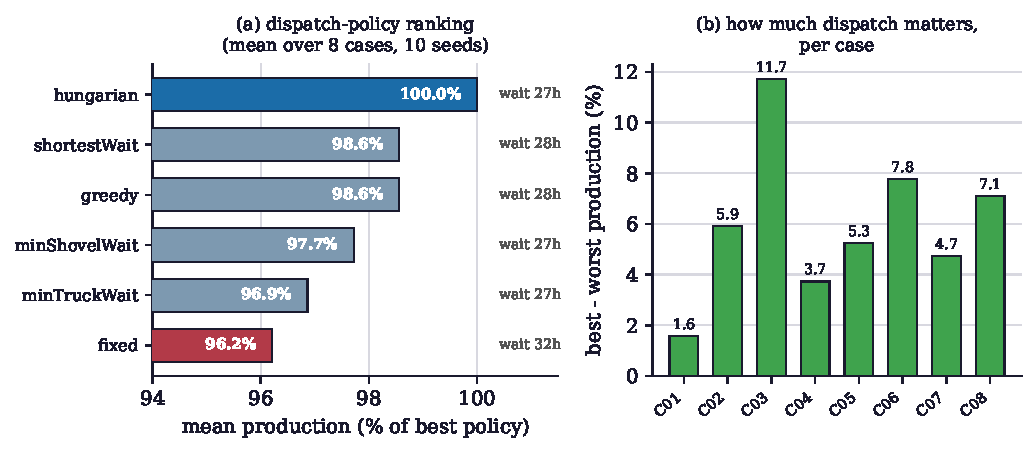
\includegraphics[width=0.84\textwidth]{fig-policies.pdf}
\caption{The measured value of dispatch, over eight cases and ten seeds with common random numbers.
\textbf{(a)} The six policies ranked by mean production as a percentage of the best: the Hungarian optimal
assignment leads, the greedy and expected-wait heuristics are within $1.4\%$ of it, and fixed assignment trails
by $3.8\%$ (with the longest truck waits). \textbf{(b)} The best-minus-worst production gain per case: dispatch
is worth from $1.6\%$ (a balanced fleet where any policy suffices) to $11.7\%$ (an imbalanced case where a good
assignment matters), a few percent in the typical case.}
\label{fig:policies}
\end{figure*}

The engine is a deterministic discrete-event simulator with next-event time advance, an integer-tick clock, and
a total event ordering by \texttt{(time, priority, sequence)}, so a run is bit-deterministic. Truck travel time
is not a constant but is computed from rimpull-versus-grade physics (total resistance is grade plus rolling
resistance), and the stochastic elements (payload, load time, dump time) are drawn from named, seeded streams. A
policy is a function from the current pit state to the next shovel for a returning truck. The six policies span
the spectrum: \emph{fixed} assignment (each truck bound to one shovel), \emph{greedy} (send the truck to the
shovel that will finish serving it earliest), \emph{shortest-expected-wait}, \emph{min-shovel-wait} and
\emph{min-truck-wait} (the two classic queue-balancing heuristics), and the \emph{Hungarian} optimal assignment,
which solves the full truck-to-shovel assignment as a minimum-cost matching~\cite{kuhn} at each decision epoch.

The engine is validated two ways. A $1\times1$ configuration, one truck and one shovel, has a closed-form
steady-state throughput, and the simulator reproduces it exactly, confirming the cycle bookkeeping. And
match-factor theory~\cite{burt,morgan}, the classical ratio of truck arrival rate to shovel service rate that
predicts fleet balance, is reproduced by the simulator's controls, confirming the queueing behaviour. Only on that
validated engine are the policies compared, and they are compared with common random numbers: for each of eight
cases and ten seeds, all six policies run against the identical random realisation, so the production difference
between two policies is a paired quantity.

\section{How Much Dispatch Matters}\label{sec:results}

The result is Fig.~\ref{fig:policies} and Table~\ref{tab:policies}. Ranked by mean production over the eight
cases, the Hungarian optimal assignment produces the most tonnes (the $100\%$ reference); below it, the
expected-wait and greedy heuristics are essentially tied at $98.6\%$, the
two queue-balancing heuristics follow at $96.9$--$97.7\%$, and naive fixed assignment is last at $96.2\%$, also
with the longest truck waits ($32$ hours against the optimal policy's $27$). The main result is the size of the
spread: fixed assignment trails the Hungarian policy by $3.8\%$ on average, and the per-case spread between the
best and worst policy (Fig.~\ref{fig:policies}b) ranges from $1.6\%$, in a well-balanced fleet where the
assignment barely matters, to $11.7\%$, in an imbalanced case where sending trucks to the right shovel is worth
real tonnes. Two conclusions follow. First, dispatch matters, a few percent of production is a large sum at mine scale, and in the
worst-balanced case it is more than a tenth. Second, most of that gain is cheap: the simple greedy policy captures
all but $1.4\%$ of what the operations-research-optimal Hungarian assignment achieves, so the marginal value of
full optimisation over a sensible myopic rule is small, and a mine gets most of the benefit from any non-trivial
policy. The paired common-random-numbers design is what separates these percent-level differences from noise.

\begin{table}[!t]
\centering
\caption{Dispatch policies ranked by mean production (percent of the best) and median truck wait, over eight
cases and ten seeds with common random numbers.}
\label{tab:policies}
\footnotesize
\setlength{\tabcolsep}{4pt}
\begin{tabular}{@{}l r r@{}}
\toprule
Policy & production (\% of best) & median wait (h) \\
\midrule
Hungarian (optimal assignment) & $100.0$ & $26.8$ \\
Shortest expected wait         & $98.6$  & $27.6$ \\
Greedy (earliest completion)   & $98.6$  & $28.4$ \\
Min shovel wait                & $97.7$  & $27.1$ \\
Min truck wait                 & $96.9$  & $27.3$ \\
Fixed assignment               & $96.2$  & $31.7$ \\
\bottomrule
\end{tabular}
\end{table}

\section{Learning the Dispatch}\label{sec:learned}

\begin{figure}[!t]
\centering
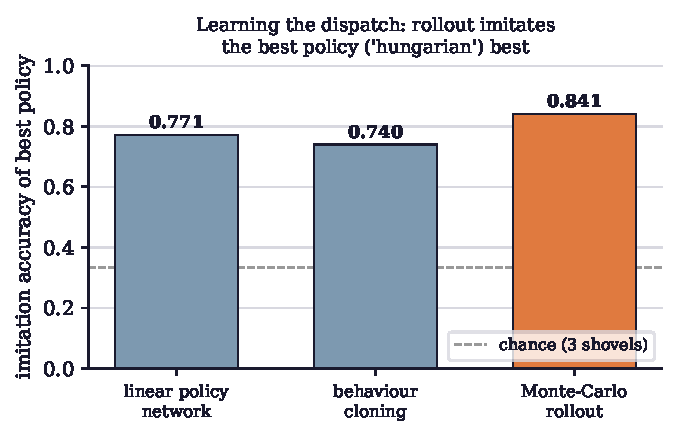
\includegraphics[width=0.86\columnwidth]{fig-learned.pdf}
\caption{Learning to dispatch. Imitation accuracy of the best classical policy (the Hungarian assignment) by
three learned dispatchers: a linear policy network ($0.771$), behaviour cloning ($0.740$), and a Monte-Carlo
rollout dispatcher ($0.841$), all well above the three-shovel chance rate of $0.33$. The rollout, which simulates
a few steps ahead under each candidate assignment before committing, imitates the optimal policy best.}
\label{fig:learned}
\end{figure}

Can the dispatch be learned? Figure~\ref{fig:learned} reports three attempts to imitate the best classical policy
(the Hungarian assignment), evaluated as the fraction of decision epochs where the learned dispatcher chooses the
same shovel. A linear policy network over six state features reaches $0.771$, straightforward behaviour cloning
$0.740$, and a Monte-Carlo rollout dispatcher~\cite{bertsekas}, which simulates a short horizon ahead under each
candidate shovel before committing, reaches $0.841$, all far above the $0.33$ three-shovel chance rate. That the
rollout imitates the optimal policy best is expected, since it approximates the same lookahead the optimal
assignment implicitly performs, and it sets the ceiling here: since the Hungarian assignment is already
near-optimal and the greedy heuristic is within $1.4\%$ of it, a learned dispatcher's practical upside over a simple heuristic is
bounded by the same few percent the policy comparison revealed: on this problem, the bench leaves no large
production gain for a cleverer policy to unlock.

\section{Discussion and Scope}\label{sec:discuss}

The bench's answer to the title question is: a few percent, typically, and up to a tenth in an imbalanced
fleet, with most of that gain captured by any sensible non-trivial policy and only a further percent or two
available from full optimisation. The size of the gain depends on how imbalanced the fleet is to begin with,
which points as much to fleet sizing as to dispatch. The methodological contribution is the paired,
validated design: common random numbers to measure percent-level differences without drowning them in variance,
and a closed-form oracle plus match-factor theory to anchor the engine. DispatchLab is a policy-comparison
\emph{sandbox}, not a production dispatch system (Modular DISPATCH, Wenco, MineStar and the
like) and not in-plant fleet tracking. The mine is synthetic and physics-grounded but has never been validated
against a real operation, because no public, ground-truthed cycle-log benchmark exists; the numbers describe the
behaviour of the model, not a prediction for a specific mine. The bench states the same scope on every panel.

\section{Conclusion}

Measured on a validated, deterministic discrete-event bench with common random numbers, truck-to-shovel dispatch
matters by a few percent of production in the typical case and up to $11.7\%$ in an imbalanced one, with the
operations-research-optimal Hungarian assignment on top, the simple greedy policy within $1.4\%$ of it, and naive
fixed assignment $3.8\%$ behind. A Monte-Carlo rollout dispatcher imitates the optimal policy best ($0.841$),
but its practical upside is bounded by the same modest spread. The measurement, that dispatch is worth
capturing but its gains are bounded and mostly cheap, and the paired, oracle-validated method behind it form the
contribution, obtained on a bench that is explicitly synthetic.

\appendices
\section{Reproduction}\label{app:repro}

The repository artifacts under \path{data/derived/} carry the eight cases' per-policy results
(\path{case-results.json}: median tonnes and truck wait with confidence intervals, ten seeds each under common
random numbers) and the learned-dispatcher analysis (\path{dl-learned.json}: the imitation accuracies and the
policy weights). The figure scripts under \path{manuscripts/dispatch-bench/figures/} aggregate them into the
ranking, the per-case gains, and the imitation-accuracy figure. Because the engine is deterministic and the
streams are seeded, re-running reproduces Table~\ref{tab:policies} and
Figs.~\ref{fig:policies}--\ref{fig:learned}, and the $1\times1$ oracle and match-factor controls are unit tests.

\balance

\begin{thebibliography}{00}

\bibitem{newman} A.~M. Newman, E.~Rubio, R.~Caro, A.~Weintraub, and K.~Eurek, ``A review of operations research
in mine planning,'' \emph{Interfaces}, vol.~40, no.~3, pp.~222--245, 2010. doi:10.1287/inte.1090.0492.

\bibitem{alarie} S.~Alarie and M.~Gamache, ``Overview of solution strategies used in truck dispatching systems
for open pit mines,'' \emph{International Journal of Surface Mining, Reclamation and Environment}, vol.~16,
no.~1, pp.~59--76, 2002. doi:10.1076/ijsm.16.1.59.3408.

\bibitem{kuhn} H.~W. Kuhn, ``The Hungarian method for the assignment problem,'' \emph{Naval Research Logistics
Quarterly}, vol.~2, no.~1--2, pp.~83--97, 1955. doi:10.1002/nav.3800020109.

\bibitem{burt} C.~N. Burt and L.~Caccetta, ``Equipment selection for surface mining: A review,''
\emph{Interfaces}, vol.~44, no.~2, pp.~143--162, 2014. doi:10.1287/inte.2013.0732.

\bibitem{morgan} W.~C. Morgan and L.~L. Peterson, ``Determining shovel-truck productivity,'' \emph{Mining
Engineering}, vol.~20, pp.~76--80, 1968.

\bibitem{glasserman} P.~Glasserman and D.~D. Yao, ``Some guidelines and guarantees for common random numbers,''
\emph{Management Science}, vol.~38, no.~6, pp.~884--908, 1992. doi:10.1287/mnsc.38.6.884.

\bibitem{bertsekas} D.~P. Bertsekas and D.~A. Casta\~non, ``Rollout algorithms for stochastic scheduling
problems,'' \emph{Journal of Heuristics}, vol.~5, no.~1, pp.~89--108, 1999. doi:10.1023/A:1009634810396.

\end{thebibliography}

\end{document}
